%%
% The BIThesis Template for Bachelor Graduation Thesis
%
% 北京理工大学毕业设计开题报告 —— 使用 XeLaTeX 编译
%
% Copyright 2020 Spencer Woo
%
% This work may be distributed and/or modified under the
% conditions of the LaTeX Project Public License, either version 1.3
% of this license or (at your option) any later version.
% The latest version of this license is in
%   http://www.latex-project.org/lppl.txt
% and version 1.3 or later is part of all distributions of LaTeX
% version 2005/12/01 or later.
%
% This work has the LPPL maintenance status `maintained'.
%
% The Current Maintainer of this work is Spencer Woo.
%
% This work consists of the files main.tex, misc/cover.tex and
% the external PDF misc/reviewTable.pdf

\documentclass[UTF8,AutoFakeBold,AutoFakeSlant,12pt]{ctexart}
\usepackage[a4paper,left=3cm,right=2.4cm,top=2.6cm,bottom=2.38cm,includeheadfoot]{geometry}
\usepackage{fontspec}
\usepackage{setspace}
\usepackage{graphicx}
\usepackage{fancyhdr}
\usepackage{titlesec}
\usepackage{pdfpages}
\usepackage{cite}
\usepackage{setspace}

% 随机生成文字,可以删掉
\usepackage{lipsum}

% 在这里替换你的姓名、专业、学院、指导老师…
\newcommand{\deptName}{计算机学院}
\newcommand{\majorName}{计算机科学与技术}
\newcommand{\className}{07xxxxxx}
\newcommand{\yourName}{惠计算}
\newcommand{\mentorName}{张哈希}
\newcommand{\offCampusMentorName}{刘阿贝尔}

% 中文大写日期(理论上这里 \ctexset{today=big} 应该就可以实现中文日期的
% 显示,但是在 misc/cover.tex 中进行这样的设置之后就是渲染不出来,暂时使
% 用即将 deprecated 的 API)
\CTEXoptions[today=big]

% 将西文字体设置为 Times New Roman
\setromanfont{Times New Roman}

%% 将中文楷体设置为 SIMKAI.TTF(如果需要)
% \setCJKfamilyfont{zhkai}{[SIMKAI.TTF]}
% \newcommand*{\kaiti}{\CJKfamily{zhkai}}

% 设置引用
\newcommand{\upcite}[1]{\textsuperscript{\cite{#1}}}

% 设置各级标题格式
\setcounter{tocdepth}{2}
\setcounter{secnumdepth}{2}

%%
% 设置一级标题、二级标题格式
% 一级标题:小三,宋体,加粗,段前段后各半行
\ctexset{section={
  format={\raggedright \bfseries \songti \zihao{-3}},
  beforeskip = 28bp plus .2ex minus .2ex,
  afterskip = 24bp plus .2ex,
  fixskip = true,
  name = {,.\quad}
  }
}
% 二级标题:小四,宋体,加粗,段前段后各半行
\ctexset{subsection={
  format = {\bfseries \songti \raggedright \zihao{-4}},
  beforeskip =28bp plus .2ex minus .2ex,
  afterskip = 24bp plus .2ex,
  fixskip = true,
  }
}

%%
% 文档开始
\begin{document}

% 报告封面

\title{\BIThesis{}研究生学位论文\LaTeX{}模板\\快速使用指南}
\author{北京理工大学~~研究生院}

\maketitle


% 评审表
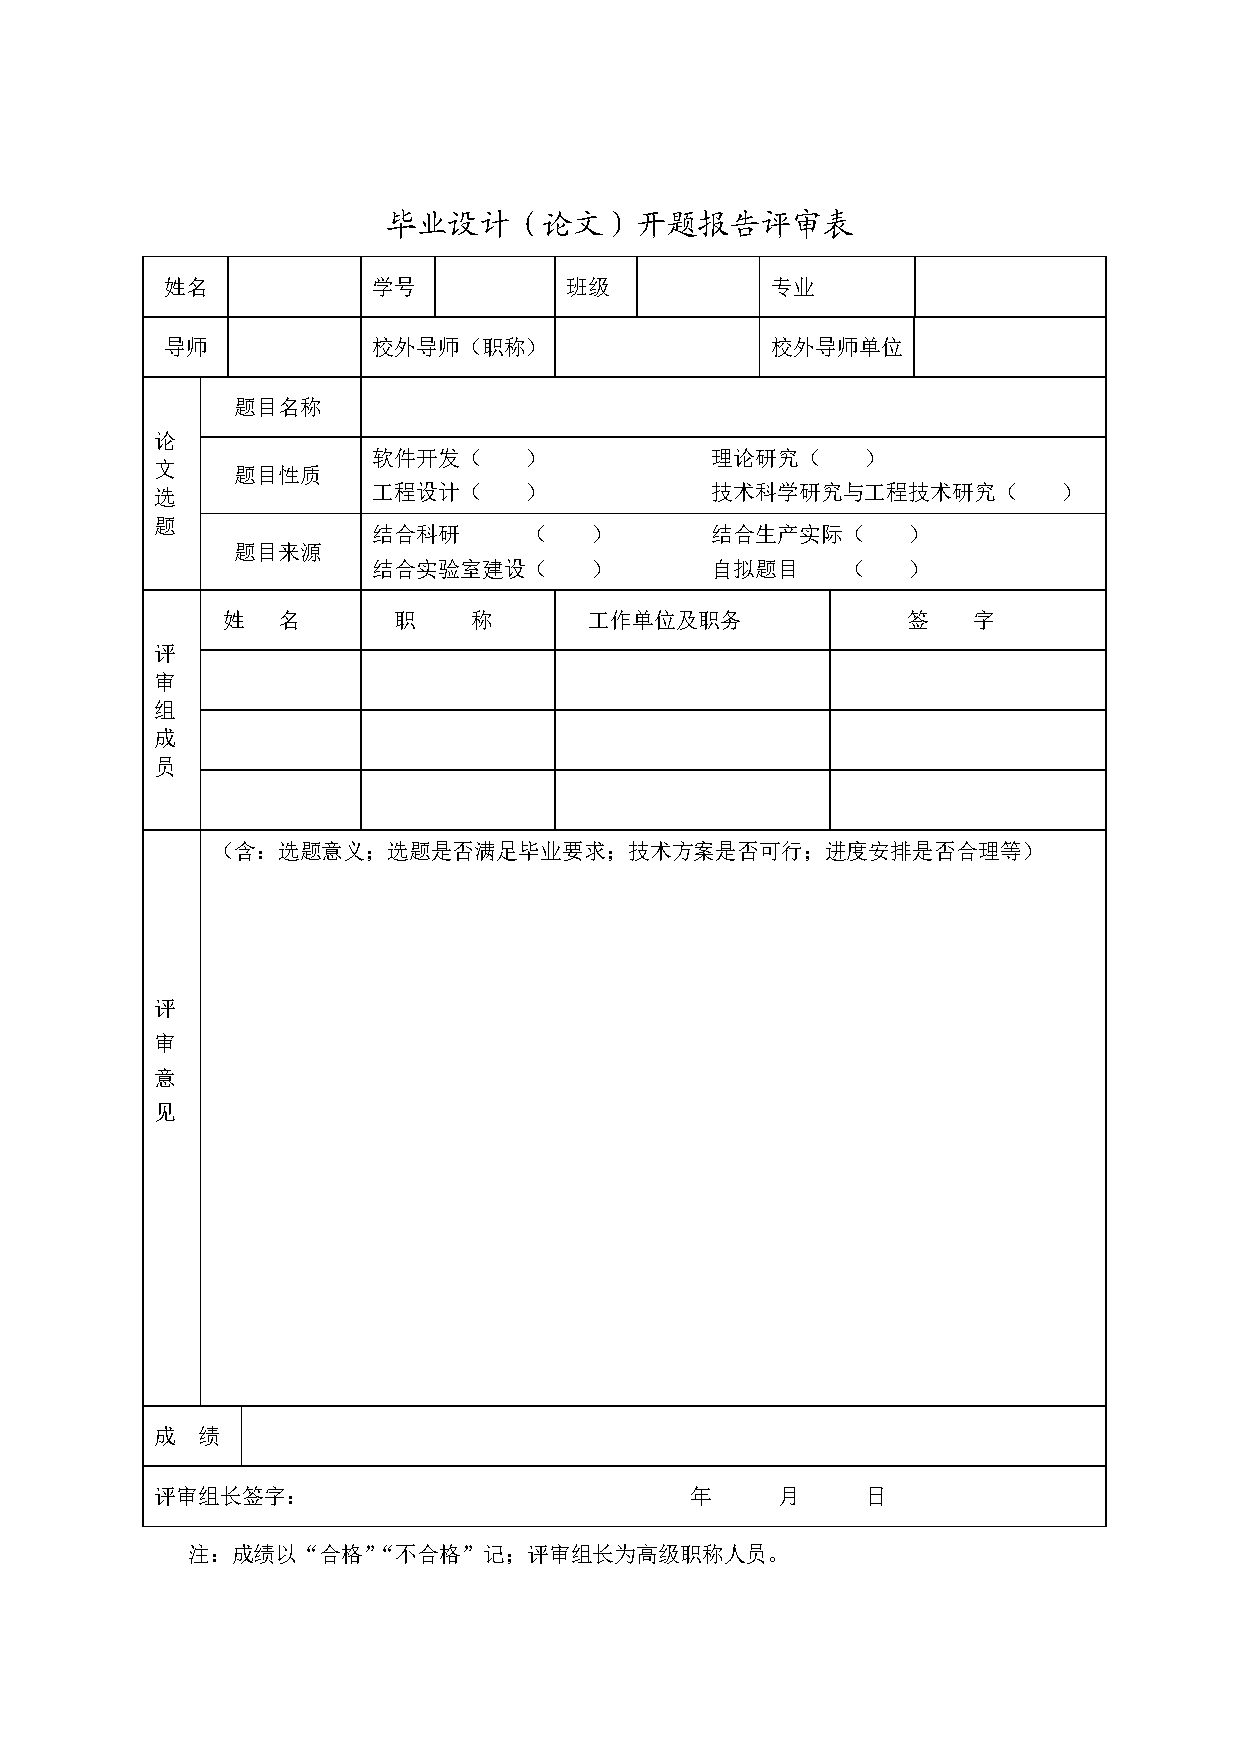
\includepdf[pages=-]{misc/reviewTableBlank.pdf}

%%
% 正文开始
\pagestyle{fancy}
% 正文从第一页开始计算页码
\setcounter{page}{1}
% 页眉和页脚(页码)的格式设定
\fancyhf{}
\fancyhead[R]{\fontsize{10.5pt}{10.5pt}\selectfont{北京理工大学本科生毕业设计(论文)开题报告}}
\fancyfoot[R]{\fontsize{9pt}{9pt}\selectfont{\thepage}}
\renewcommand{\headrulewidth}{1pt}
\renewcommand{\footrulewidth}{0pt}

% 正文 22 磅的行距
\setstretch{1.53}
% 正文首行悬挂 1.02cm
\setlength{\parindent}{1.02cm}

% 内容开始
\section{毕业设计(论文)选题的内容}
\lipsum[1]

\section{研究方案}
\subsection{本选题的主要任务}
\lipsum[2]

\subsection{技术方案的分析、选择}
\lipsum[3-5]

\subsection{实施技术方案所需的条件}

\subsection{存在的主要问题和技术关键}
目前存在的主要问题是

\subsection{预期能够达到的研究目标}

\section{课题计划进度表}

\section{参考文献}

\end{document}
